\documentclass[10pt,a4paper]{article}

\usepackage[margin=1.65cm,top=1.4cm,bottom=1.5cm]{geometry}
\usepackage{amsmath,amssymb}
\usepackage{graphicx}
\usepackage{booktabs}
\usepackage{xcolor}
\usepackage[hidelinks]{hyperref}
\usepackage{caption}
\usepackage{titlesec}

\captionsetup{font=small,labelfont=bf,skip=2pt}
\titleformat{\section}{\normalfont\bfseries}{\thesection}{0.6em}{}
\titlespacing*{\section}{0pt}{5pt}{1pt}
\setlength{\parskip}{2.5pt plus 1pt}
\setlength{\parindent}{0pt}
\setlength{\abovedisplayskip}{3pt}\setlength{\belowdisplayskip}{3pt}
\setlength{\abovedisplayshortskip}{1pt}\setlength{\belowdisplayshortskip}{2pt}
\setlength{\textfloatsep}{6pt plus 2pt}

\newcommand{\code}[1]{\texttt{#1}}
\newcommand{\topk}{\operatorname{TopK}}
\newcommand{\PH}[1]{\textcolor{red}{[#1]}}

\begin{document}

{\centering
{\large\bfseries A surrogate for the carried code: RBLapSum on the branch, the carry left hard}\\[1pt]
{\small 8-layer TinyStories models of the K+J notes, \code{code\_residual}, abs-TopK over \(N=1536\), \(T=2\), MD optimizer; one seed.
Runs \code{be\_cr\_*} (box bergen), configs \code{configs/cr\_kj/carry/}, scopes \code{rblapsum\_surrogate\_scope=carry\_*}.}\par}


\section{The problem}

With the code carried between blocks (\code{code\_residual}) hard Top-\(K'\) gains \(0.06\)--\(0.075\) nats at every
\(K'\) and RBLapSum (\(K\) active, pool \(K{+}J\)) gains \(-0.03\) to \(+0.015\): at a matched active count the
surrogate is worth \(0.047\) at \(K=32\), loses \(0.02\)--\(0.03\) at \(K=128,256\), and its backward is the unstable
part of the grid (\code{docs/kj-vs-hard-topk-code-residual.tex}).  The first-order scope removes the instability with
a second backward pass and is \emph{worse} than the unmodified surrogate at every \(K=32\) cell (\(+0.007\) to
\(+0.017\) at 20k).  This note locates the conflict and removes it at no cost.

\section{Where the probabilities act}

Gate \(\ell\) reads \(u_\ell=c_\ell+v_\ell\) (carried code plus the block's encoded contribution) and outputs
\(c_{\ell+1}=M_\ell u_\ell\), \(M_\ell\) the Top-\(K\) mask.  Its output has two consumers, the carry
\(u_{\ell+1}=c_{\ell+1}+v_{\ell+1}\) (a skip path) and the read \(x_{\ell+1}=\mathrm N(D_\ell c_{\ell+1})\) (a branch):
\begin{equation}
  \frac{\partial\mathcal L}{\partial u_\ell}=M_\ell\bigl(g^{\rm c}_{\ell+1}+r_{\ell+1}\bigr),\qquad
  g^{\rm c}_{\ell+1}=\frac{\partial\mathcal L}{\partial u_{\ell+1}},\quad
  r_{\ell+1}=D_\ell^{\!\top}\frac{\partial\mathcal L}{\partial(D_\ell c_{\ell+1})}
  \label{eq:hard}
\end{equation}
(at the last gate \(r\) is the unembedding's gradient).  In the stream-carried stack the gate has only the second
consumer: everything block \(\ell{+}1\) does, its own gate included, goes through \(D_\ell\).  RBLapSum relaxes the gate
as a whole, \(M_\ell\to M_\ell+S_\ell\) with the \code{through\_rank\_kappa} support term \(S_\ell\) (kernel
\(\kappa_i=e^{-|s_i-b|/T}/2T\); on the support \(S_{ii}=|u_i|\kappa_i\approx b/2T\) at the boundary).  In the stream
stack \(S_\ell\) acts on \(r_{\ell+1}\) alone and what reaches gate \(\ell{-}1\) has passed through \(E_\ell\), the block
and \(D_{\ell-1}\), which mix the coordinates.  In the code stack it also acts on \(g^{\rm c}_{\ell+1}\), which already
contains \(S_{\ell+1}g^{\rm c}_{\ell+2}\): along a coordinate near the boundary the backward multiplies \(1+|u|\kappa\)
per gate.  The carry is a residual connection in code space, trainable because its backward is the identity; a
relaxation placed on the skip path compounds.  The conflict is \emph{where} the probabilities act, not the kernel.

\section{The carry-aware surrogate}

Keep the skip path hard, relax the branch: the gate's output is split into the copy the next gate carries and the
copy the decoder reads (forward and inference unchanged), and
\begin{equation}
  \frac{\partial\mathcal L}{\partial u_\ell}=M_\ell\bigl(g^{\rm c}_{\ell+1}+r_{\ell+1}\bigr)+S_\ell^{\!\top}\hat g_{\ell+1},
  \qquad
  \hat g_{\ell+1,i}=r_{\ell+1,i}+\begin{cases}0 & \text{local}\\ H_{\ell+1,i} & \text{hard}\\ \rho R_{\ell+1,i} & \text{persistent,}\end{cases}
  \label{eq:carry}
\end{equation}
with \(H_\ell=M_\ell(r_{\ell+1}+H_{\ell+1})\) the downstream read gradients a coordinate reaches along the hard carry,
\(R_\ell=r_{\ell+1}+\rho R_{\ell+1}\) every downstream read with a survival factor \(\rho\) per gate, \(H=R=0\) above
the last gate.  The support term is driven by read gradients only, so no kernel sees another gate's support term
through the carry: the products are gone, the terms of the gates above still reach gate \(\ell\), added, through
\(M_\ell\), and carry and update receive one gradient (R1 of \code{docs/rblapsum-code-residual.tex}).  The cost is two
per-coordinate sums along the backward; no second pass.  The drivers are the first-order loss change of one flip at
gate \(\ell\) -- \(c_{\ell+1,i}\) changes by \(\pm u_{\ell,i}\), which block \(\ell{+}1\) reads, and later blocks read while
the coordinate stays in the code -- under three models of what follows.  \emph{Local} counts the next read only (the
stream stack's logic; exactly the gradient of a model whose decoder reads a relaxed gate while the carry is hard).
\emph{Hard} follows the actual downstream masks (an evicted feature's remaining run; for an inactive candidate almost
always nothing).  \emph{Persistent} lets the entering coordinate survive each further gate with probability \(\rho\).
The \emph{mixed} scope uses hard for the active members and persistent for the inactive ones; \(\rho\) is measured
below.  Unlike the first-order estimator, which needs the fully hard gradient at every gate and hence a second pass,
the carry is where the gradient is taken hard, and the reads still carry the gates above through the branch, as in the
stream stack.  (\code{rblapsum\_surrogate\_scope=carry\_local|carry\_hard|carry\_persistent|carry\_mixed},
\code{rblapsum\_carry\_decay}=\(\rho\).)

\section{Measurements}

\textbf{Setup.}  The code-carried \(T=2\) arm of the K+J grid: 8\(\times\)768, \(N=1536\), \code{residual\_out} at
every block, no output norm, batch \(96\times512\), the 20k-step cosine schedule, seed 1337.  Baselines are the grid's
runs (hard Top-\(K'\) with the post-norm, RBLapSum \code{pool}, the \code{first\_order} sweep) read at matching steps;
each new scope trains the grid's config with one field changed, stopped at step 3000 by \code{train\_guard.py
--stop-step} (schedules untouched).  Step 3000 is where the grid's surrogate margins are largest and already of their
final sign (\code{pool}: \(-0.061\to-0.042\) from 3k to 20k at \(K=32\), \(+0.048\to+0.034\) at \(K=256\)); two cells
are continued to 10k steps.

\begin{figure}[t]
\centering
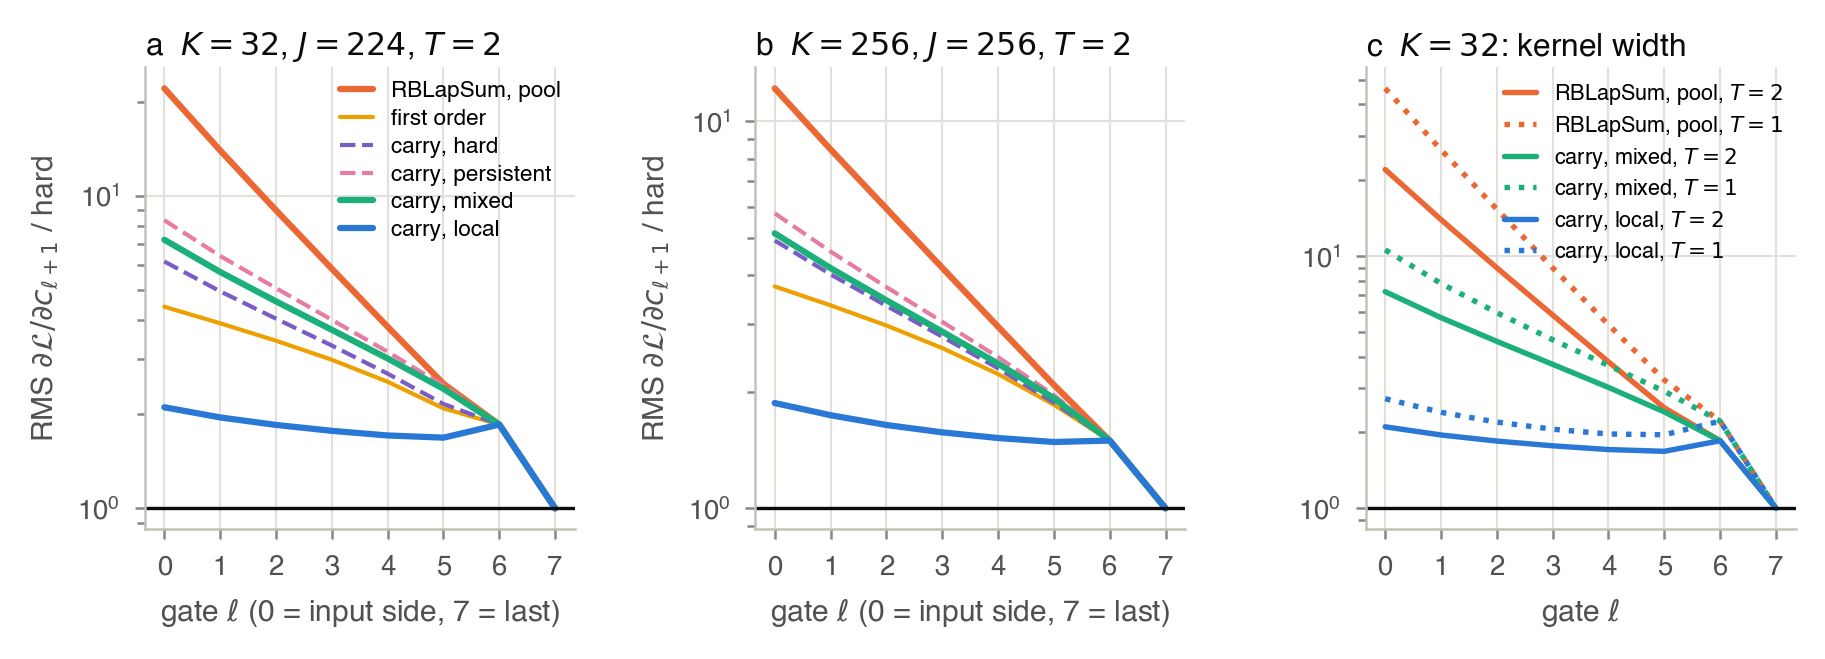
\includegraphics[width=.72\textwidth]{figures/carry/fig_init.png}
\caption{\textbf{Backward along the carried code at initialization}: RMS \(\partial\mathcal L/\partial c_{\ell+1}\)
at each gate's output relative to the hard backward of the same weights (\code{analysis/surrogate\_probe.py}, 4
validation sequences).  Under \code{pool} the gradient grows \(\times1.5\) (\(K{=}32\)) and \(\times1.4\) (\(K{=}256\))
per gate toward the input, \(22\times\) and \(12\times\) hard at gate 0 (\(46\times\) at \(T{=}1\), dotted); every carry
scope and the first-order estimator grow additively, one term per gate, the local scope staying within \(2.1\times\).}
\label{fig:init}
\end{figure}

\textbf{At initialization} (Fig.~\ref{fig:init}) the surrogate's share of the gradient energy at the gates,
\(\sigma=\lVert S^\top\hat g\rVert^2/\lVert m\odot g\rVert^2\) averaged over gates, is \(0.70\) for \code{pool},
\(0.74\) for \code{carry\_mixed}, \(0.31\) for \code{carry\_local} and \(0.24\) for first order at \(K=32\)
(\(0.30\), \(0.20\), \(0.09\), \(0.09\) at \(K=256\)): the mixed scope injects as much support signal as the unmodified
backward, as a sum instead of a product.

\textbf{Runs of the carried code} (Fig.~\ref{fig:runs}; \code{analysis/code\_runs.py}, 16 validation sequences, hard
forward).\label{sec:runs}  The carry is persistent for a subset of the code, not for the code.  In the trained hard
Top-32 model every gate evicts \(30\)--\(54\%\) of the support it receives; a feature that enters is still there one
gate later with probability \(0.51\), two gates later \(0.34\); \(12\%\) of the final code was carried from gate 0 and
\(54\%\) entered at the last gate (hard Top-256: \(0.57\), \(0.41\), \(17\%\), \(34\%\)).  An entry at gate 0 is read
by \(2.7\)--\(3.1\) blocks on average, against 8 under the persistent model and 1 under the local one.  The \code{pool}
surrogate trains the model \emph{out of} the carry: at \((32,224)\) turnover is \(63\%\) per gate at step 4000 and
\(70\%\) at 20k, one-gate survival \(0.21\to0.16\), and \(77\%\) of the final code enters at the last gate -- the
stream stack's re-selection at every block, reproduced by a model that has a carry.  This is why the carry was
``nearly neutral'' for the surrogate in the grid.

\begin{figure}[t]
\centering
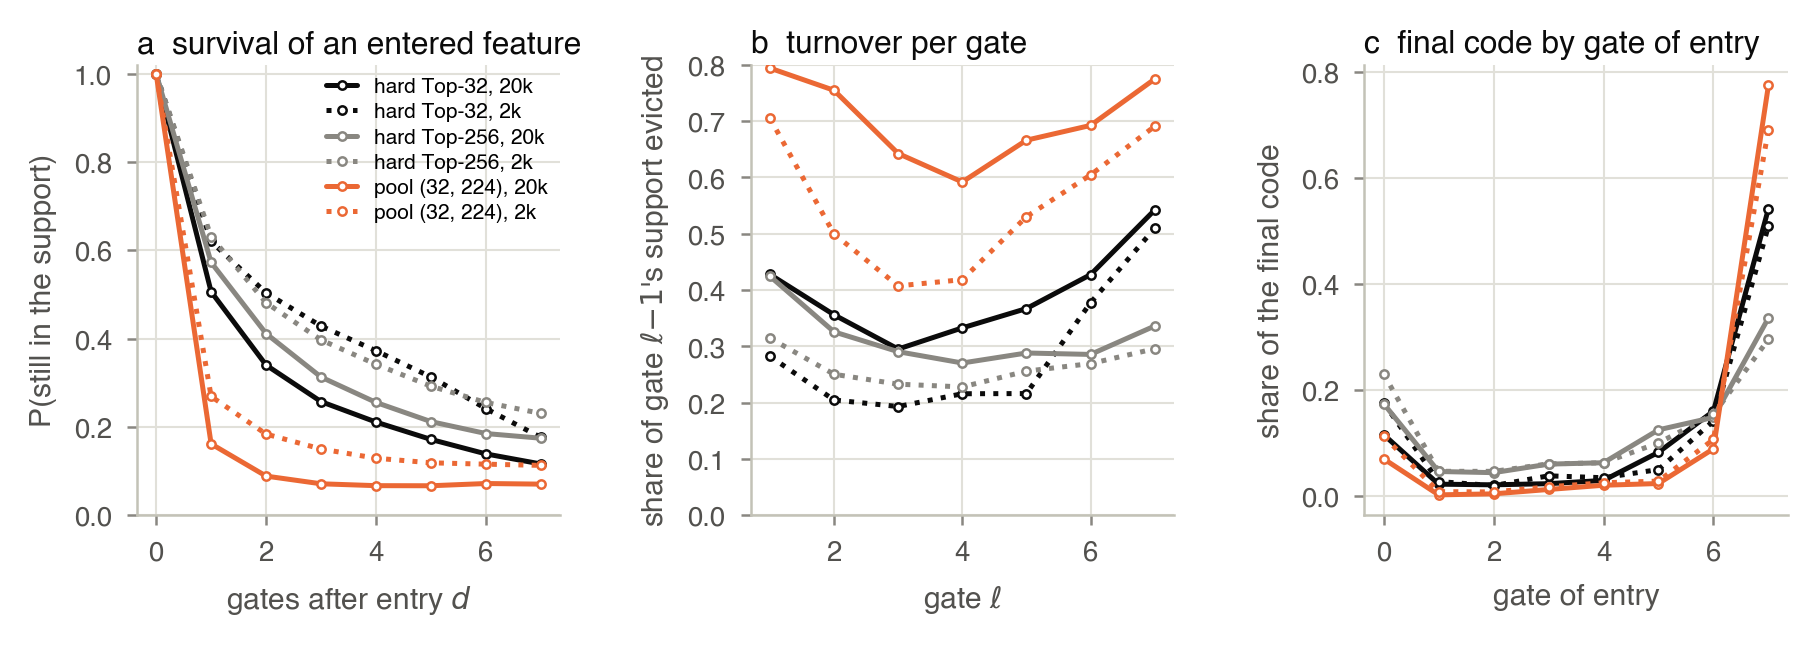
\includegraphics[width=.72\textwidth]{figures/carry/fig_runs.png}
\caption{\textbf{Runs of the carried code.}  \textbf{a} Probability that a feature which entered the support is
still in it \(d\) gates later.  \textbf{b} Share of the support gate \(\ell\) receives from gate \(\ell{-}1\) that it
evicts.  Hard baselines at steps 4000 and 20000, the \code{pool} and first-order cells, and the carry scopes at step 3000.}
\label{fig:runs}
\end{figure}

\textbf{Training} (Fig.~\ref{fig:screens}, Table~\ref{tab:screens}).  At \(K=32\), \(J=224\) the \emph{local} scope ends
step 3000 at \(-0.058\) below hard Top-32, where the unmodified surrogate is at \(-0.061\) and the first-order
estimator at \(-0.033\); it leads \code{pool} by \(0.02\) at step 1000 and the two coincide from step 2000.  The
\emph{mixed} scope ends at \(-0.118\), twice the margin of the unmodified surrogate and the margin of hard Top-128
over hard Top-32 at the same step (\(-0.124\)): with 32 active features it reaches the hard model that activates 128,
\(1.782\) against \(1.776\), and is below hard Top-64 (\(1.835\)) from step 500 on.  Neither run's gradient norm
exceeded 1 (the \code{pool} cell spiked four times, to 3.3); both have the hard model's feature usage (usage entropy
\(0.79\); hard \(0.73\), first order \(0.79\), \code{pool} \(0.59\)) and the hard model's use of the carry
(Fig.~\ref{fig:runs}: one-gate survival \(0.52\) and \(0.53\) at step 3000, turnover \(35\%\) and \(33\%\), against
\(0.60\)/\(31\%\) for hard Top-32 and \(0.21\)/\(63\%\) for \code{pool}).  The local scope (like first order)
places its turnover at the top -- \(13\)--\(25\%\) of the support replaced at gates 1--4, \(67\)--\(79\%\) at the last
two, \(79\%\) of the final code entering at the last gate -- while the mixed scope has the hard model's profile
(\(25\)--\(49\%\) at every gate, \(49\%\) of the final code from the last gate, \(12\%\) carried from gate 0).  The gain of the unmodified surrogate at \(K=32\) is thus not bought by the
products along the carry: a backward without them keeps the gain, keeps the carry, and with the downstream reads in
the entry term doubles the gain.

At \(K=256\), \(J=256\), where the unmodified surrogate is the pathological case (\(+0.047\) above hard Top-256 at
step 3000, \(+0.034\) at 20k, its code turning over \(46\%\) per gate against the hard model's \(28\%\)), the local scope ends
step 3000 at \(+0.009\), and the gap closes steadily (\(+0.065\), \(+0.030\), \(+0.016\), \(+0.009\) at steps 500,
1000, 2000, 3000, against \(+0.133\), \(+0.087\), \(+0.057\), \(+0.048\) for \code{pool}); the hard baseline carries
the post-norm, worth about \(0.007\) to a hard model in the stream grid, and the surrogate cells do not.  The local
model's code is the hard model's again -- one-gate survival \(0.57\), turnover \(30\%\) per gate, usage entropy
\(0.94\) (hard: \(0.62\), \(28\%\), \(0.93\); \code{pool}: \(0.40\), \(46\%\), \(0.89\)) -- and its gradient norm never
exceeded 1.  The mixed scope goes further: \(+0.005\) at step 1000, below hard Top-256 from step 2000 and
\(-0.0045\) at 3000 (\(1.736\) against \(1.741\)) -- a surrogate with 256 active features ahead of the hard model with
the same count, which no code-carried cell of the grid achieved -- with hard Top-512 at \(-0.037\); its code is
the hard model's too (survival \(0.61\), turnover \(30\%\), \(17\%\) of the final code carried from gate 0).
\PH{K=128; the 10k continuations}

\begin{figure}[t]
\centering
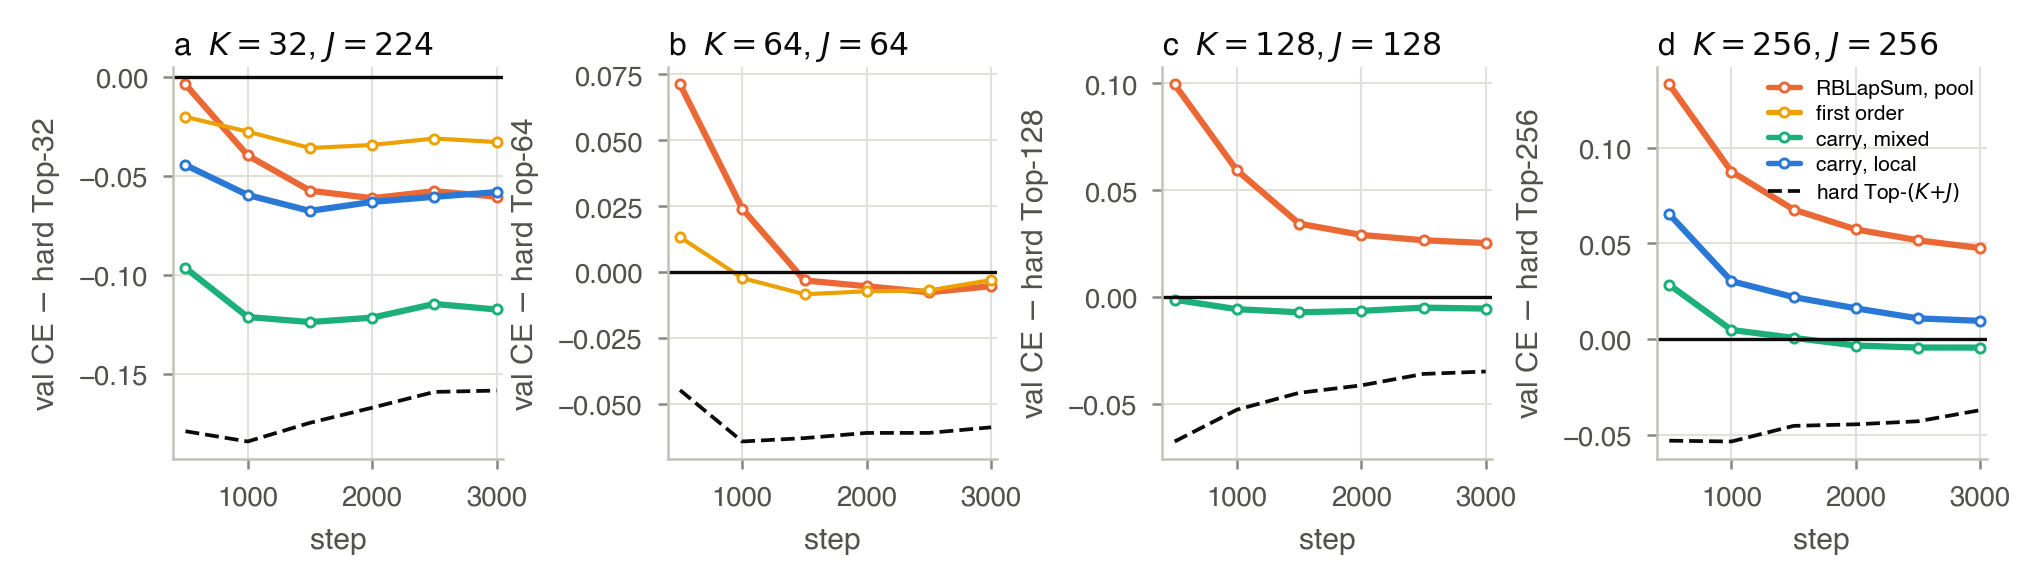
\includegraphics[width=\textwidth]{figures/carry/fig_screens.png}
\caption{\textbf{Validation CE relative to hard Top-\(K\)} (code carried, post-norm) during the first 3000 steps,
one panel per \((K, J)\); the dashed line is hard Top-\((K{+}J)\), the model that activates the whole pool.  \PH{}}
\label{fig:screens}
\end{figure}

\begin{table}[t]
\centering\small
\begin{tabular}{llccccccc}
\toprule
 & & \multicolumn{7}{c}{validation CE at step 3000, minus hard Top-\(K\) (code carried, post-norm)} \\
\cmidrule(lr){3-9}
\(K\) & \(J\) & pool & first order & carry local & carry mixed & mixed, \(\rho{=}0.5\) & carry persistent & hard Top-\((K{+}J)\) \\
\midrule
32 & 224 & \(-0.061\) & \(-0.033\) & \(-0.058\) & \(\mathbf{-0.118}\) & \PH{} & -- & \(-0.158\) \\
128 & 384 & \(+0.016\) & \PH{} & \PH{} & \PH{} & -- & -- & \(-0.072\) \\
256 & 256 & \(+0.047\) & \PH{} & \(+0.009\) & \(\mathbf{-0.005}\) & \PH{} & \PH{} & \(-0.037\) \\
\bottomrule
\end{tabular}
\caption{Step-matched validation CE after 3000 steps, each cell minus the code-carried hard Top-\(K\) baseline of its
row (hard Top-32 \(1.899\), Top-128 \(1.776\), Top-256 \(1.741\)); \code{pool} and first order are the grid's own runs
read at step 3000.  Bold: below every other surrogate of the row.}
\label{tab:screens}
\end{table}


\section{What the measurements show}

\textbf{The conflict is the placement, not the kernel.}  RBLapSum relaxes a gate whose output, in the code-carried
stack, is also a skip connection, and the relaxation is multiplied along the skip path, \((1+b/2T)\) per gate
(Fig.~\ref{fig:init}).  Putting the probabilities where they were in the stream-carried stack -- on what the decoder
reads -- and leaving the carry's backward the mask removes the product exactly, in one backward pass, with one gradient
for carry and update.  Trained, the local scope keeps the unmodified surrogate's whole gain at \(K=32\) (first order,
which also removes the product but at the price of a second pass, keeps half of it) and removes four fifths of its
loss at \(K=256\), without a gradient spike in either cell.

\textbf{The carry gives the surrogate something the stream stack could not: a downstream for the entry term.}  In
the stream stack a candidate that enters at gate \(\ell\) is re-encoded by gate \(\ell{+}1\), so the next read is all
there is to evaluate it against.  In the code stack an entering feature is carried, and the first-order value of
letting it in is the sum of the reads it would reach.  The mixed scope evaluates the inactive candidates on that sum
(\(\rho=1\)) and the active members on the reads their run actually reaches, and it doubles the gain at \(K=32\)
(\(-0.118\): 32 active features at the loss of hard Top-128) and turns the loss at \(K=256\) into a gain
(\(-0.005\) below hard Top-256, a model with the same active count).  Its surrogate energy equals the unmodified
backward's (\(\sigma=0.74\) against \(0.70\) at \(K=32\)), delivered as a sum of single-flip terms instead of a
product: the unmodified backward was not too strong, it was multiplying.

\textbf{The surrogate-trained model uses the carry only when the surrogate leaves it alone.}  The trained hard
models carry about half of their support from gate to gate (one-gate survival \(0.5\)--\(0.6\), \(26\)--\(39\%\)
turnover); the \code{pool}-trained ones re-select \(46\)--\(70\%\) of it at every gate and end with the stream stack's
code, which is why the carry was worth nothing to them.  Every carry-scope model has the hard model's survival and
turnover (Fig.~\ref{fig:runs}): the surrogate's support signal and the carry's persistence add instead of
competing, and the measured survival (\(\rho\approx0.5\)) is also the natural value for the persistent chain
(\PH{cm05}).

\textbf{Scope.}  One seed, one configuration family (8 layers, \(N=1536\), \(T=2\), no output norm), screens of
3000 steps with step-matched 20k-step baselines trained on a different machine of the same GPU generation; the
grid's own early-versus-final margins (\(-0.061\to-0.042\) at \(K=32\), \(+0.048\to+0.034\) at \(K=256\) for
\code{pool}) are the only calibration of what a 3000-step difference becomes.  \PH{long runs}

\end{document}
